\documentclass[9pt,twocolumn,twoside]{gsajnl}
% Use the documentclass option 'lineno' to view line numbers
\usepackage{booktabs}
\usepackage{siunitx}
\usepackage{adjustbox}
\usepackage{geometry}
\articletype{gos} % article type

\title{Nucleotide Diversity Loss on a Plant Y Chromosome Following Recent Recombination Suppression}

\author[$\ast$,$\dagger$,1]{Josh Hough}
\author[$\dagger$]{Wei Wang}
\author[$\dagger$]{Spencer C.H. Barrett}
\author[$\dagger$]{Stephen I. Wright}

\affil[$\ast$]{Department of Plant Sciences, University of California, Davis}
\affil[$\dagger$]{Department of Ecology and Evolutionary Biology, University of Toronto}

%\affil[$\dagger$]{Author two affiliation}
%\affil[$\ddagger$]{Author three affiliation}
%\affil[$\S$]{Author four affiliation}
%\affil[$\ast\ast$]{Author five affiliation}

\keywords{Sex Chromosome Evolution; Nucleotide Diversity; Recombination; Deleterious Mutations}

\runningtitle{Plant sex chromosome evolution} % For use in the footer

\correspondingauthor{Josh Hough}

\begin{abstract}
X and Y chromosomes differ in effective population size ($N_{e}$), rates of recombination, and exposure to natural selection, all of which can affect levels of genetic diversity. On Y chromosomes with suppressed recombination, selection is expected to eliminate neutral variation and reduce the $N_{e}$ of Y compared to X chromosomes or autosomes. However, non-selective factors including female biased sex ratios and high variance in male reproductive success can also reduce Y-linked $N_{e}$, making it difficult to infer the causes of low Y-diversity. Here, we investigate the factors affecting levels of polymorphism within the genome during sex chromosome evolution in \textit{Rumex hastatulus} (Polygonaceae), a dioecious plant with young sex chromosomes. Strikingly, we find that neutral diversity for genes on the Y is on average \textasciitilde 2.1\% of the value for their homologues on the X, corresponding to a chromosome-wide reduction of \textasciitilde 93\% compared to the neutral expectation. We demonstrate that the magnitude of this diversity loss is inconsistent with a reduced male $N_{e}$ caused by neutral processes including female-biased sex ratios and high variance in male reproductive success. Instead, using forward simulations, we show that the loss of diversity on the Y can be explained by interference among a large number ($\geq$ 800 Kb) of weakly selected mutations. Our results are in agreement with theory on "interference selection", and provide evidence that the effects of purifying selection over a large number of genetically-linked sites can substantially reduce neutral diversity. Given the recent origin of \textit{R. hastatulus} sex chromosomes (\textasciitilde 15MYA), our results imply that Y chromosome degeneration in the early stages may be largely driven by interference rather than positive selection for gene silencing followed by neutral genetic drift.
\end{abstract}


\setboolean{displaycopyright}{true}

\begin{document}

\maketitle
\thispagestyle{firststyle}
\marginmark
\firstpagefootnote
\correspondingauthoraffiliation{jhough@ucdavis.edu}
\vspace{-11pt}

\section*{Introduction}

\lettrine[lines=2]{\color{color2}M}{}orphologically distinct sex chromosomes have evolved multiple times independently in both plants and animals \citep{westergaard1958,ohno1967,bull1983,charlesworth1991,charlesworth2015plant}. Despite clear biological differences between these kingdoms, X and Y chromosomes in both lineages have undergone similar genetic changes. For example, in both groups the loss of recombination between X and Y chromosomes has been associated with an accumulation of deleterious mutations and a gradual loss of genes from the Y chromosome \citep{hough2014,bergero2015,bachtrog2013NRG}, and in some species, the degeneration of the Y has led to the evolution dosage compensation of the X chromosome \citep{charlesworth1996CB,muyle2012,mank2013sex,papadopulos2015}. The independent evolution of these phenomena in such taxonomically distant groups suggest that general evolutionary mechanisms may be involved, but inferring the causes of molecular evolution and patterns of polymorphism in genomic regions that lack recombination is a longstanding challenge for both theoreticians and experimentalists \citep{charlesworth1978,feldman1980evolution,barton1995general,charlesworth1996CB,otto1997deleterious,charlesworth2000degeneration,mcvean2000effects}.

One fundamental difference between the X and Y chromosomes is that there are 1/3 as many Y-linked gene copies as X-linked ones in a diploid population. Thus, genes on the Y chromosome are expected to experience an effective population size ($N_{e}$) that is 1/4 that of autosomal genes, whereas the  $N_{e}$ for genes on the X chromosome should be 3/4 that of autosomal genes (assuming an equal number of reproducing females and males). The lowered $N_{e}$ of the Y chromosome implies that that the equilibrium level of neutral polymorphism - proportional to the product of $N_{e}$ and the neutral mutation rate, $\mu$ - should be lower for Y-linked genes than for their X-linked counterparts. In the absence of recombination, genes on the Y chromosome are also expected to be in strong linkage disequilibrium, making them vulnerable to diversity loss due to selection against strongly deleterious mutations (background selection) and selective sweeps of strongly beneficial mutations (genetic hitchhiking). Furthermore, the build-up of linkage disequilibrium between selected mutations on the Y means that selection will act non-independently across the chromosome, such that selection at a focal site may "interfere" with selection at sites with which it is linked \citep{hill1966HReffect}. A large body of work has now shown that in theory such "selective interference" effects can substantially reduce both the efficacy of selection and the level of neutral variability \citep{fisher1930genetical, muller1964relation, hill1966HReffect, mcvean2000,KaiserCharlesworth,good2014genetic}. These arguments all suggest that non-recombining Y chromosomes should harbor a lower amount of neutral genetic variability than predicted based on the number of Y chromosomes in a population, but the extent to which background selection, genetic hitchhiking, or selective interference have affected chromosome-wide levels of diversity in natural populations, and the relative importance of these processes, is not well-understood.

In addition to reduced diversity arising from selection, in species with female-biased sex ratios or extensive male-male competition, high variance in male reproductive success is also expected reduce the $N_{e}$ experience by genes on the Y chromosome \citep{caballero1995,charlesworth2001,laporte2002,pool2007,ellegren2009}, suggesting that inferences about the effects positive of purifying selection need to be distinguished from these neutral processes. Because variance in male reproductive success reduces both Y-linked $N_{e}$ and autosomal $N_{e}$ \citep{kimura1964number,nomura2002effective}, evidence for this can therefore be obtained by comparing levels of neutral diversity on X and Y chromosomes relative to values on autosomes. For example, high variance in male reproductive success causes a reduction in the Y/A diversity ratio, but an increase in the X/A ratio. Based on such comparisons, studies in humans, for example, have suggested that the inflated X/A ratio is due to a historical excess of breeding females compared to males \citep{hammer2008sex} (and see \citep{bustamante2009,hammer2010,cotter2016genetic}).

Despite widespread interest in determining the evolutionary factors affecting neutral diversity on sex chromosomes \citep{ellegren2011,bachtrog2013NRG}, we know very little about the influence of sex ratio variation or linked selection in determining levels of diversity on more recently evolved sex chromosomes. The time scales over which these different effects are likely to be important is therefore not well understood. In humans, estimates of Y-linked diversity are considerably lower than predicted under neutral models, and simulations suggest that levels of diversity are consistent with strong purifying selection \citep{Wilsonsayres2014}. However, given that human sex chromosomes evolved from autosomes \textasciitilde 200 million years ago (MYA) \citep{lahn1999four,ross2005dna}, is not immediately obvious whether purifying selection might have such strong effects on Y chromosomes that evolved \textit{do novo} from autosomes over much more recent evolutionary time (e.g., within the last \textasciitilde 20 MYA in the case of plants \citep{charlesworth2015plant}). Y-linked diversity loss might on the one hand be expected to be lower in younger systems due to a shorter history of recombination suppression. On the other hand, simulations of strong selection models (background selection and genetic hitchhiking) suggest that these processes may have the greatest effects during the earliest stages of sex chromosome evolution, before the Y has lost many of its genes \citep{bachtrog2008temporal}. Moreover, there is clear evidence from simulation studies that even weak purifying selection, if acting non-independently across large number of sites, can generate substantial deviations from neutrality, whereas classic background selection theory breaks down in such cases \citep{mcvean2000, comeron2002population, KaiserCharlesworth, good2014genetic}. Given that a large number of sites are likely to be in linkage disequilibrium on a recently evolved Y chromosome, such "interference selection" \textit{sensu} \citep{good2014genetic} is a good candidate model for exploring the evolutionary dynamics of young plant sex chromosomes.

To investigate the factors affecting nucleotide diversity in the early stages of sex chromosome evolution, we analyzed neutral polymorphism levels on X, Y, and autosomal chromosomes in the plant \textit{R. hastatulus }(Polygonaceae). This species is a dioecious annual with heteromorphic X and Y chromosomes that evolved \textasciitilde 15 MYA \citep{quesada2011,grabowska2015,navajas2005}, making Y chromosomes in this species over 100 million years younger than the highly degenerated Y chromosomes in mammals \citep{lahn1999,ross2005dna}. \textit{Rumex hastatulus} has also received particular attention because of the occurrence of an interesting polymorphic in sex chromosome system, in which both XY and $XY_{1}XY_{2}$ males occur in geographically distinct populations ( so-called "chromosomal races") \citep{smith1963mechanism}. The $XY_{1}XY_{2}$ sex chromosome system in this species is thought to have originated through an X-autosome fusion, with the XY system maintaining the ancestral chromosome complement \citep{smith1964evolving}. Despite the recent origin of sex chromosomes in both races, there is evidence that both Y's have undergone gene loss and functional deterioration \citep{hough2014}. Here, to simplify our comparison of polymorphism levels on X, Y, and autosomes, we focus only on the ancestral Y chromosome, which occurs in both sex chromosome races.

Of particular importance for our study, \textit{R. hastatulus} populations have also been found to consistently exhibit female-biased reproductive sex ratios, with a mean sex ratio of $N_{f}/(N_{m}+N_{f})=0.6$ \citep{pickup2013influence}. Female-biased sex ratios are not uncommon in dioecious plants with heteromorphic X and Y chromosomes \citep{field2013comparative,hough2013evolutionarily}, and their occurrence in \textit{R. hastatulus} provides an excellent opportunity to investigate both the demographic and selective factors contributing to sex-linked variability.

\section*{Materials and Methods}
\subsection*{Population Samples and Sex-Linked Genes}
We analyzed sex-linked and autosomal genes identified from Illumina RNA sequence data from 12 males and 12 females (1 male and 1 female from each of 6 populations). Samples were collected in 2010 from throughout the native range of \textit{R. hastatulus} (locations in Table S1), and plants were grown in the glasshouse at the University of Toronto from seeds collected from open-pollinated females. We extracted RNA from leaf tissue using Spectrum Plant Total RNA kits (Sigma-Aldrich). Isolation of mRNA and cDNA synthesis was conducted according to standard Illumina RNAseq procedures, and sequencing was conducted on two Illumina HiSeq lanes with 150-bp end reads at the Genome Quebec Innovation Center. Reads from these samples were mapped to the \textit{R. hastatulus} reference transcriptome \citep{hough2014} using the Burrows–Wheeler Aligner \citep{li2010fast}, followed by Stampy \citep{lunter2011stampy}. We used Picard tools (http://picard.sourceforge.net) to process mapping alignments for the Genome Analysis Toolkit \citep{mckenna2010genome} variant calling software, and subsequently removed genes with low coverage (<10x) and low Phred Quality Scores <20. The population samples analyzed here were previously reported in Hough et al. (2014), where they were used to validate the ascertainment of sex-linked genes identified through segregation analysis, and raw sequences are available from the GenBank Short Read Archive under accession no. SRP041588. Here, to consider sex linked genes that were identified in all of our sequenced population samples, we focused on the previously described set of 460 X/Y genes for which a Y homolog was found in both the Texas and North Carolina races (i.e., X/Y genes where the Y copy was inferred to be on the $Y_{1}$ chromosome).

\subsection*{Autosomal Genes}
In evaluating evidence for nucleotide diversity differences between X and Y chromosomes, it is important to distinguish between reduced Y-linked diversity, and the possibility that X-linked diversity is elevated above the level predicted from a neutral model. To do this, we normalized our sex-linked diversity estimates by autosomal diversity, and compared empirical X/A and Y/A nucleotide diversity ratios to those predicted from neutral models and from simulations (described below). Because the criteria for ascertaining autosomal loci in Hough et al. (2014) were based on identifying four segregating SNPs per locus, and since this set of genes is likely to be higher in diversity than the average autosomal gene, here we instead used the larger set of all non-sex linked (putatively autosomal) genes as our autosomal reference. We filtered genes in this set to remove any genes that may have been sex-linked but were not identified as such by Hough et al.'s conservative ascertainment criteria. In particular, we removed: (i) any genes in which there was evidence for at least one SNP with a sex-linked segregation pattern, (ii) any genes where SNPs showed fixed heterozygosity in males and fixed homozygosity in females, (iii) genes with less than 10X coverage or greater than 100X coverage from independently obtained genomic coverage data (to filter out duplicates or genes with highly repetitive sequences), and (iv) any genes containing SNPs with large (>0.4) allele frequency differences between males and females. Finally, we removed genes with fewer than 100 synonymous sites to avoid biasing our results toward genes that may have been particularly short due to assembly problems. This filtering resulted in a final set of 12,356 autosomal genes.

\subsection*{Phasing X and Y alleles}
To estimate polymorphism for X and Y sequences separately, it is necessary to infer the phase of SNPs in sex-linked transcripts in males. In previous work, phasing alleles on \textit{R. hastatulus} sex chromosomes was achieved using segregation analysis from a genetic cross. Here, to phase SNPs from population samples where such segregation data was unavailable, we used HAPCUT \citep{bansal2008hapcut}, a maximum-cut based algorithm that reconstructs haplotypes using sequenced fragments (Illumina read data) from the two homologous chromosomes to output a list of phased haplotype blocks containing the SNP variants on each chromosome. Because the resulting haplotype blocks produced by HAPCUT contained SNPs that were phased relative to each other, but not designated to either the X or Y chromosome, we assigned individual variants to X or Y by independently identifying fixed X-Y differences within each haplotype block (i.e., sites where all females were homozygous, and all males were heterozygous). Identifying such fixed differences within phased haplotype blocks enabled us to then infer the correct phase (X or Y) of the polymorphisms from HAPCUT’s output. In particular, this was done by matching the phase of fixed X-Y differences with their neighboring polymorphic sites: when a fixed X-Y difference occurred in the same phased haplotype block as a polymorphic site, then the polymorphic variants in that block were assigned to either X or Y based on the known phase of the fixed difference with which they were matched. SNPs that were identified outside of phased blocks, or in blocks without fixed X-Y differences, were recorded as missing data. Finally, we filtered out SNPs with coverage > 60, QUAL score > 60, and those within a distance of 10bp or less from indels. This filtering procedure resulted in fasta-formatted alignments of X and Y sequences for 372 sex-linked genes.

We further validated the results of HAPCUT’s allele phasing by comparing the accuracy of this method with the phasing-by-segregation method that was conducted in Hough et al. (2014). To do this, we first phased the sequence data from parents and their progeny using HAPCUT’s algorithm (using the same parameters as for the population data), and then identified cases where SNPs were inferred on the Y chromosome by HAPCUT, but where the true level polymorphism, obtained from the genetic cross, was zero. We identified 7 \% of sex-linked genes that either had  phasing errors of this kind genotyping errors. This corresponds to a SNP error rate estimate of 1.7 x 10-4. Note that this rate is very low relative to population-based estimates of polymorphism on the X and autosomes (Table 1), and therefore should have minimal effects on our estimation of the X/A ratio. However, because this rate is high relative to the expected level of polymorphism on the Y chromosome, we further filtered genes in which we found evidence for false-positive SNP calls arising from: (i) phasing errors caused by gene duplicates (more than two haplotypes), (ii) polymorphisms around indels, and (iii) genotyping errors caused by low Y-expression. This final filtering was conducted by manually checking each individual putative polymorphism on the Y chromosome using IGV \citep{robinson2011integrative}.

\subsection*{Estimating nucleotide diversity on sex chromosomes and autosomes}
For each locus in our analysis, we calculated Watterson’s (1975) estimator of the population parameter $\theta=4N_{e}\mu$, where $N_{e}$ is the effective population size, and $\mu$ is the mutation rate \citep{watterson1975}, using a modified version of the Perl program Polymorphurama \citep{bachtrog2006}. To compare sex-linked and autosomal loci, we calculated the average value of $\theta$, weighted by the number of synonymous sites in each gene (\X Figure 2). We obtained 95\% confidence intervals for X/A and Y/A ratios by bootstrapping per gene using the BCa method \citep{efron1994} implemented in the Boot package in R \citep{canty2012boot}, and calculating X/A and Y/A on each iteration for 20000 replicates each. Bootstrapping was conducted on the final filtered set of 173 sex-linked, and 12355 autosomal genes. Note that the lack of recombination on the Y chromosome implies that statistical assumptions about independence across loci are violated, suggesting that the true uncertainty in the estimate Y/A may be wider than implied by bootstrapping results. To address this, we also used a maximum likelihood approach, implemented in a modified version of the MLHKA software \citep{wright2004hka}, to independently estimate a credibility interval for the Y/A ratio (Figure S1). Because of the thousands of genes involved, a likelihood method incorporating divergence to control for heterogeneity in mutation rate was not feasible, as this would require maximizing the likelihood estimate of the mutation rate for each locus independently. Therefore, we assumed no heterogeneity in mutation rate, no recombination between Y-linked genes, and free recombination between autosomal loci. Our model thus had two parameters: $\theta_{autosomal}$ and Y/A. We varied both parameters and evaluated the likelihood for Y/A from 0.001 to 1, and $\theta_{autosomal}$ from 0.001 to 0.01.

\subsection*{Neutral predictions and the effect of sex ratio bias on diversity}
To test whether our estimated levels of diversity on X, Y and autosomal chromosomes could be explained by neutral processes, we compared our estimated levels diversity to predictions from a model for the expected $N_{e}$ of males and females when the variance in offpring number is smaller or larger than the standardly assumed Poisson \citep{kimura1964number, hedrick2011genetics}. As we were primarily interested in the influence of variance in male reproductive success on Y-linked $N_{e}$, and the parameter space within which this effect might generate Y/A and X/A ratios consistent with our data, we ignored non-poission variance in female offspring numbers, and calculated male $N_{e}$ as:

\begin{equation}
N_{e_{m}}=\frac{N_{m}k_{m}-1}{k_{m}-1+\frac{V_{k_{m}}}{\overline{k}}} \label{eq:Vk}
\end{equation}

where $k_{m}$ and $V_{k_{m}}$ are the mean and variance in male offspring number, respectively, in a population of $N_{m}$ reproducing males, and $\overline{k}$ is the total mean number of progeny \citep{kimura1964number}. Given expected values of $N_e_{m}$ for a range of values for $V_{k_{m}}$ and $N_{m}$, the corresponding neutral expectation for autosomal and sex-linked $N_{e}$ at equilibrium were calculated as:

\begin{equation}
N_{e_{A}} = \frac{4N_{m}N_{f}}{N_{m}+N_{f}} \label{eq:Ne}
\end{equation}

\begin{equation}
N_{e_{X}} = \frac{9N_{m}N_{f}}{4N_{m}+2N_{f}} \label{eq:NeX}
\end{equation}

\begin{equation}
N_{e_{Y}} = \frac{N_{m}}{2} \label{eq:NeY}
\end{equation}

respectively, following \citep{wright1931evolution}. Note that with equal sex ratios $N_{f} = N_{m}$, and Poisson-distributed offspring numbers ($V_{k} = \overline{k}$), then $N_{e_{X}}/N_{e_{A}} = 0.75$, and $N_{e_{Y}}/N_{e_{A}} = 0.25$ and in the standard model. Figure 1 shows these predictions as a function of the sex ratio for a range values of $V_{k_{m}}$, and we tested the fit of our observed Y/A and X/A diversity ratios to model predictions (shown in Figure 2) assuming the empirically-estimated \textit{R. hastatulus} population sex ratio of 0.6 \citep{pickup2013influence}.

\begin{figure}[htbp]
\centering
\noindent
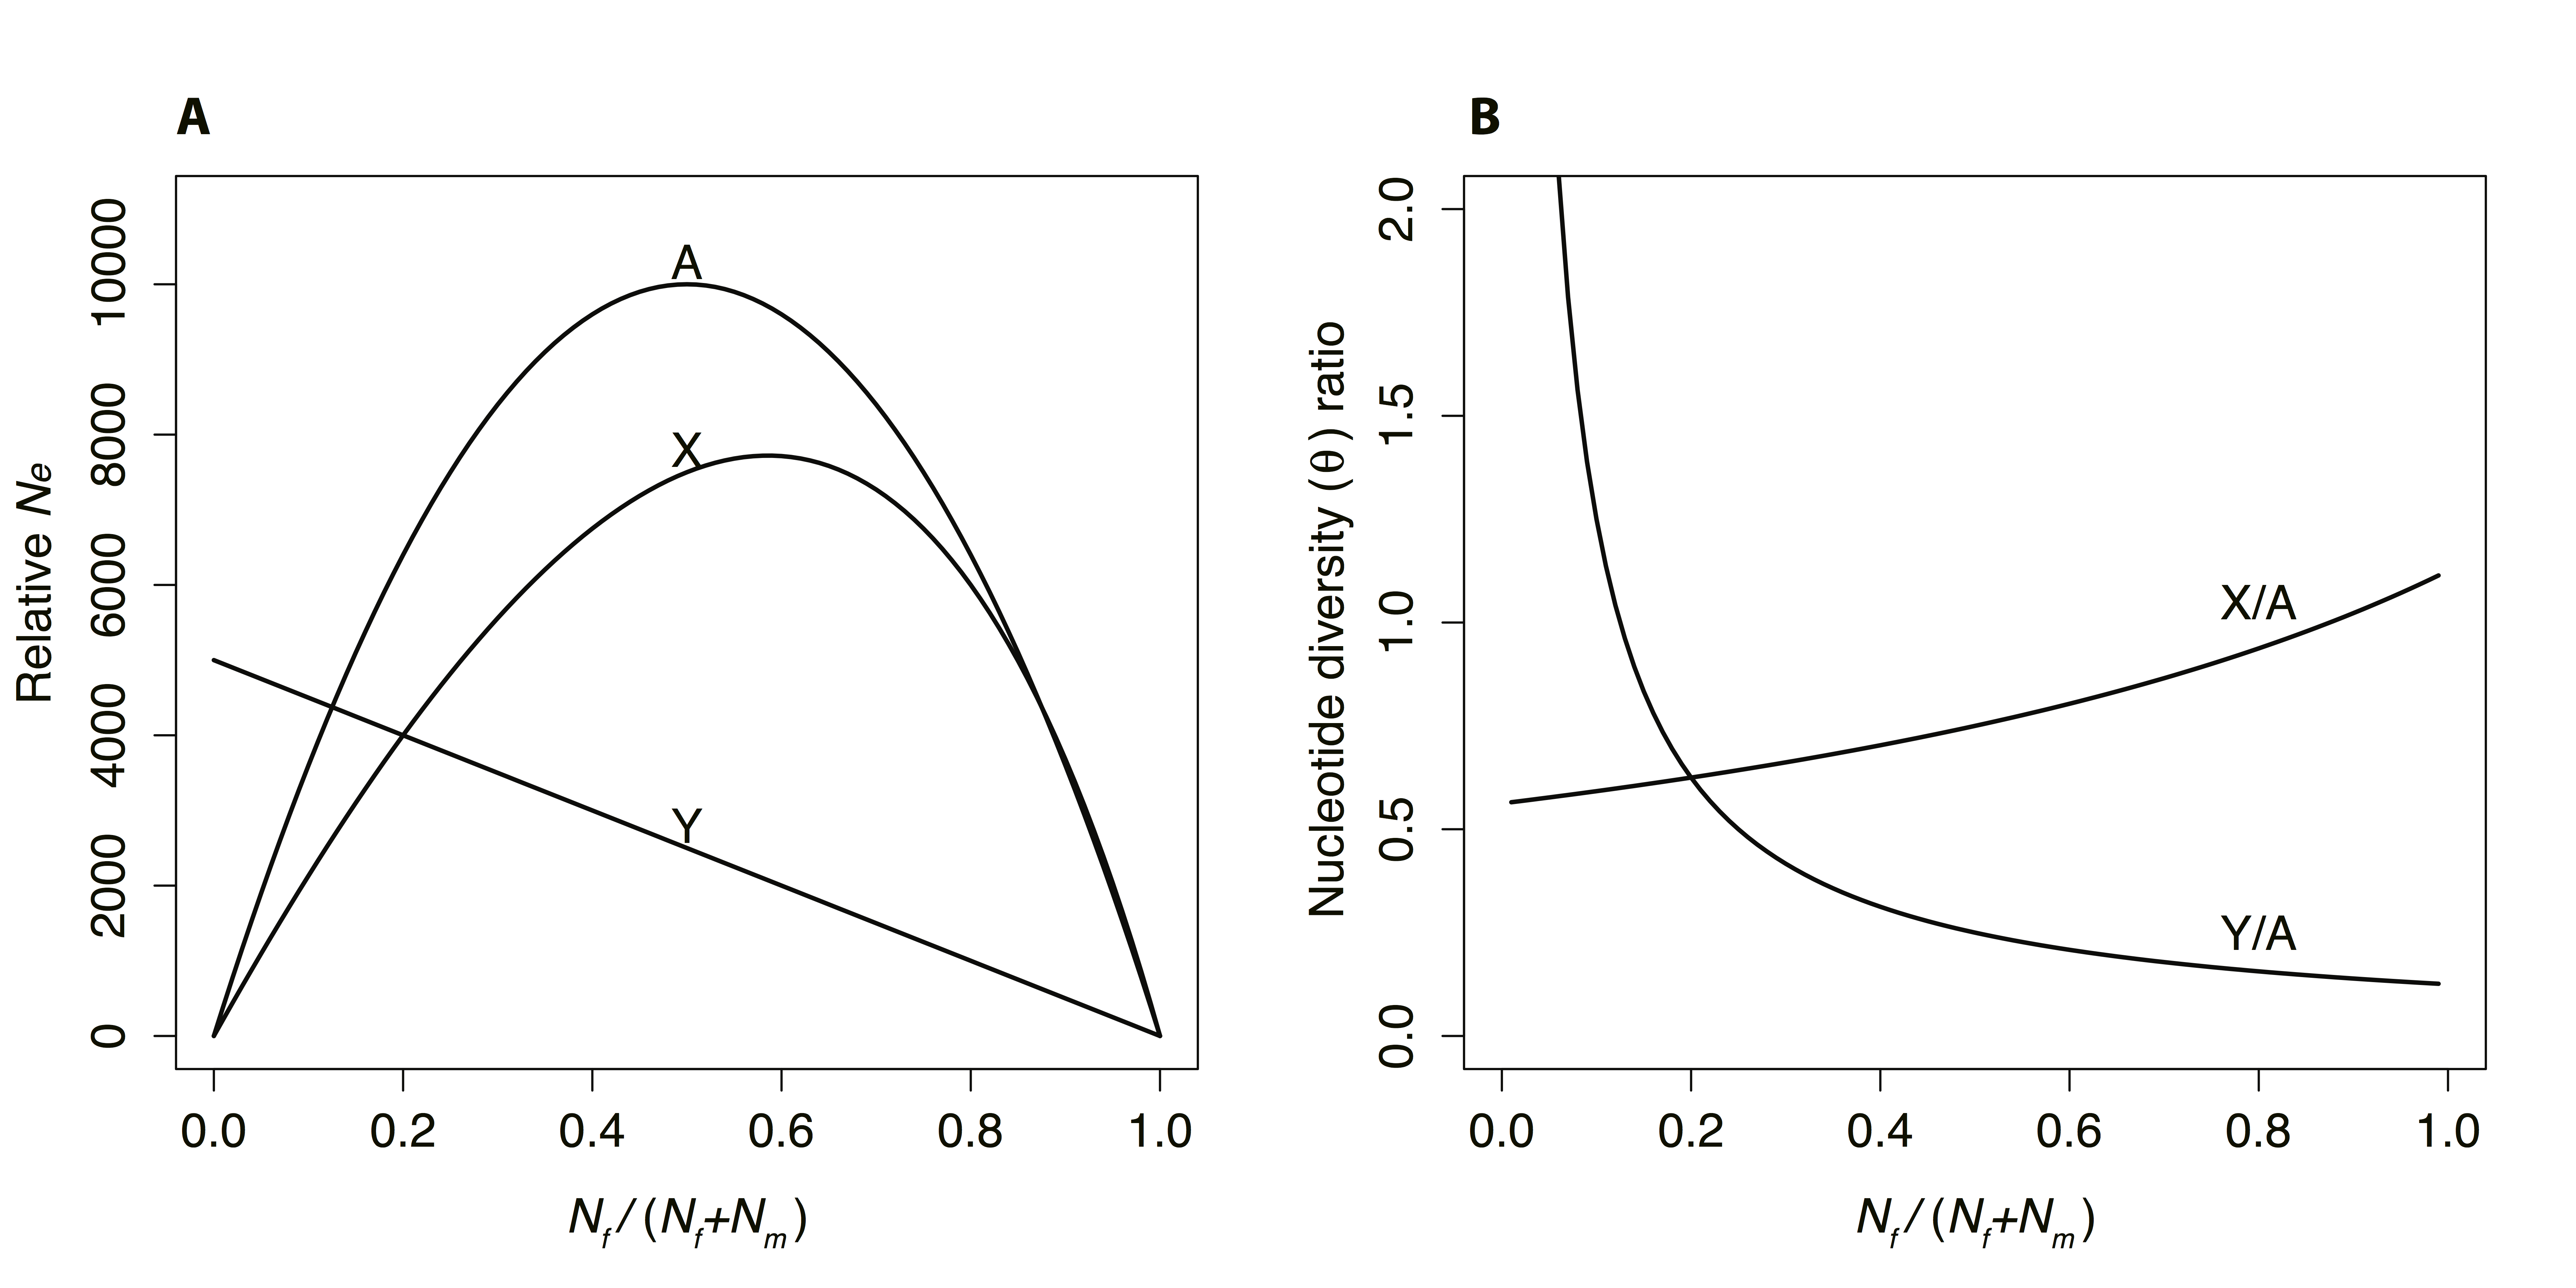
\includegraphics[width=\linewidth]{figure1.jpg}
\caption{The relation between effective population size and sex ratio bias for genes on autosomes (\textbf{A}) and the X chromosome (\textbf{B}), and corresponding normalized X/A and Y/A ratios (\textbf{C}). The sex ratio is shown as the proportion of females, $N_{f}/(N_{f}+N_{m})$, plotted against $N_{e}/N$, where $N=N_{m}+N_{f}$. Dotted curves show equilibrium predictions when both males and females produce Poisson-distributed offspring numbers and ($V_{k}$=$\overline{k}=2$). Solid curves correspond to increasing values for $V_{k_{m}}$, the variance in male offspring number, ranging from Poisson/2 (top solid curve in panels A and B) to 3*Poisson (bottom most curve). For (\textbf{C}) we assumed equal neutral mutation rates among genes and calculated the expected neutral diversity as $\theta=4N_{e}\mu$.
}
\label{fig:spectrum}
\end{figure}

\subsection*{Simulations of purifying selection}
To study the effects of purifying selection on expected levels of Y-chromosome diversity, we conducted forward-time simulations of haploid Y chromosomes using the software SFSCODE \citep{hernandez2008flexible}. We first estimated the distribution of fitness effects of deleterious mutations from our polymorphism data for X-linked genes using the method of \citep{keightley2007joint}, which fits a gamma distribution of selection coefficients to the observed frequency distribution of nonsynonymous and synonymous polymorphism. We then used this estimated gamma distribution to parameterize the simulations, initializing each with our estimated $\theta$ from autosomal genes, but appropriately adjusted to reflect the expected reduction in $N_{e}_{Y}$ for a sex ratio of $N_{f}/(N_{f}+N_{m})=0.6$. To match our sample size and the number of synonymous sites sample from our data (see Supporting Information), the simulations sampled 6 haploid chromosomes, and contained 45,331bp of linked neutral sequence from which we calculated silent site diversity. To examine the expected reduction in diversity ($\pi/\pi_{0}$) as a function of the number of selected sites ($L$), we ran simulations over a range of values of $L$, up to a maximum of 5x$10^{6}$ (Figure 3A). To estimate $L$ from our data, we calculated the approximate likelihood of our observed data based on the proportion of simulations in which synonymous diversity, $\pi__{simulated}$, was not significantly different from our empirical estimate, $\pi__{observed}$ (Figure 3B).

\section*{Results and Discussion}
\subsection*{Extensive loss of Y-chromosome diversity}
Our analysis of polymorphism levels across the genome in the dioecious plant \textit{R. hastatulus} reveals that neutral diversity on the Y chromosome is substantially lower than expected from a standard neutral model. In particular, neutral diversity on Y-linked genes $\theta_{Y}$ is on average \textasciitilde 2.1\% of the value for their homologues on the X chromosome. Talking 1/4 of the mean autosomal diversity as the equilibrium expectation under neutrality \citep{wright1931evolution}, this corresponds to a chromosome-wide reduction of \textasciitilde 93\%. Note that by comparing X and Y diversity to autosomal diversity, our results indicate that the difference between X and Y homologues is not due to an elevation of diversity on the X chromosome, but rather a Y-specific reduction. Our results do suggest a slight elevation in X-linked diversity relative to the neutral prediction of X/A=0.75, but this difference is not significantly different from the expectation for the empirically-estimated ratio of 0.6. Although our estimates of diversity have not beed normalized by divergence, previous work has shown that the average synonymous substitution rate, between \textit{R. hastatulus} and the non-dioecious outgroup \textit{R. bucephalophorus} is not significantly different for sex-linked (0.2016) or autosomal genes (0.219) \citep{hough2014}. It is therefore unlikely that our results are caused by mutation rate differences between sex-linked and autosomal genes.

\subsection*{Female biased sex ratios and variance in male offspring number}

%\begin{figure}[htbp]
%\centering
%\noindent
%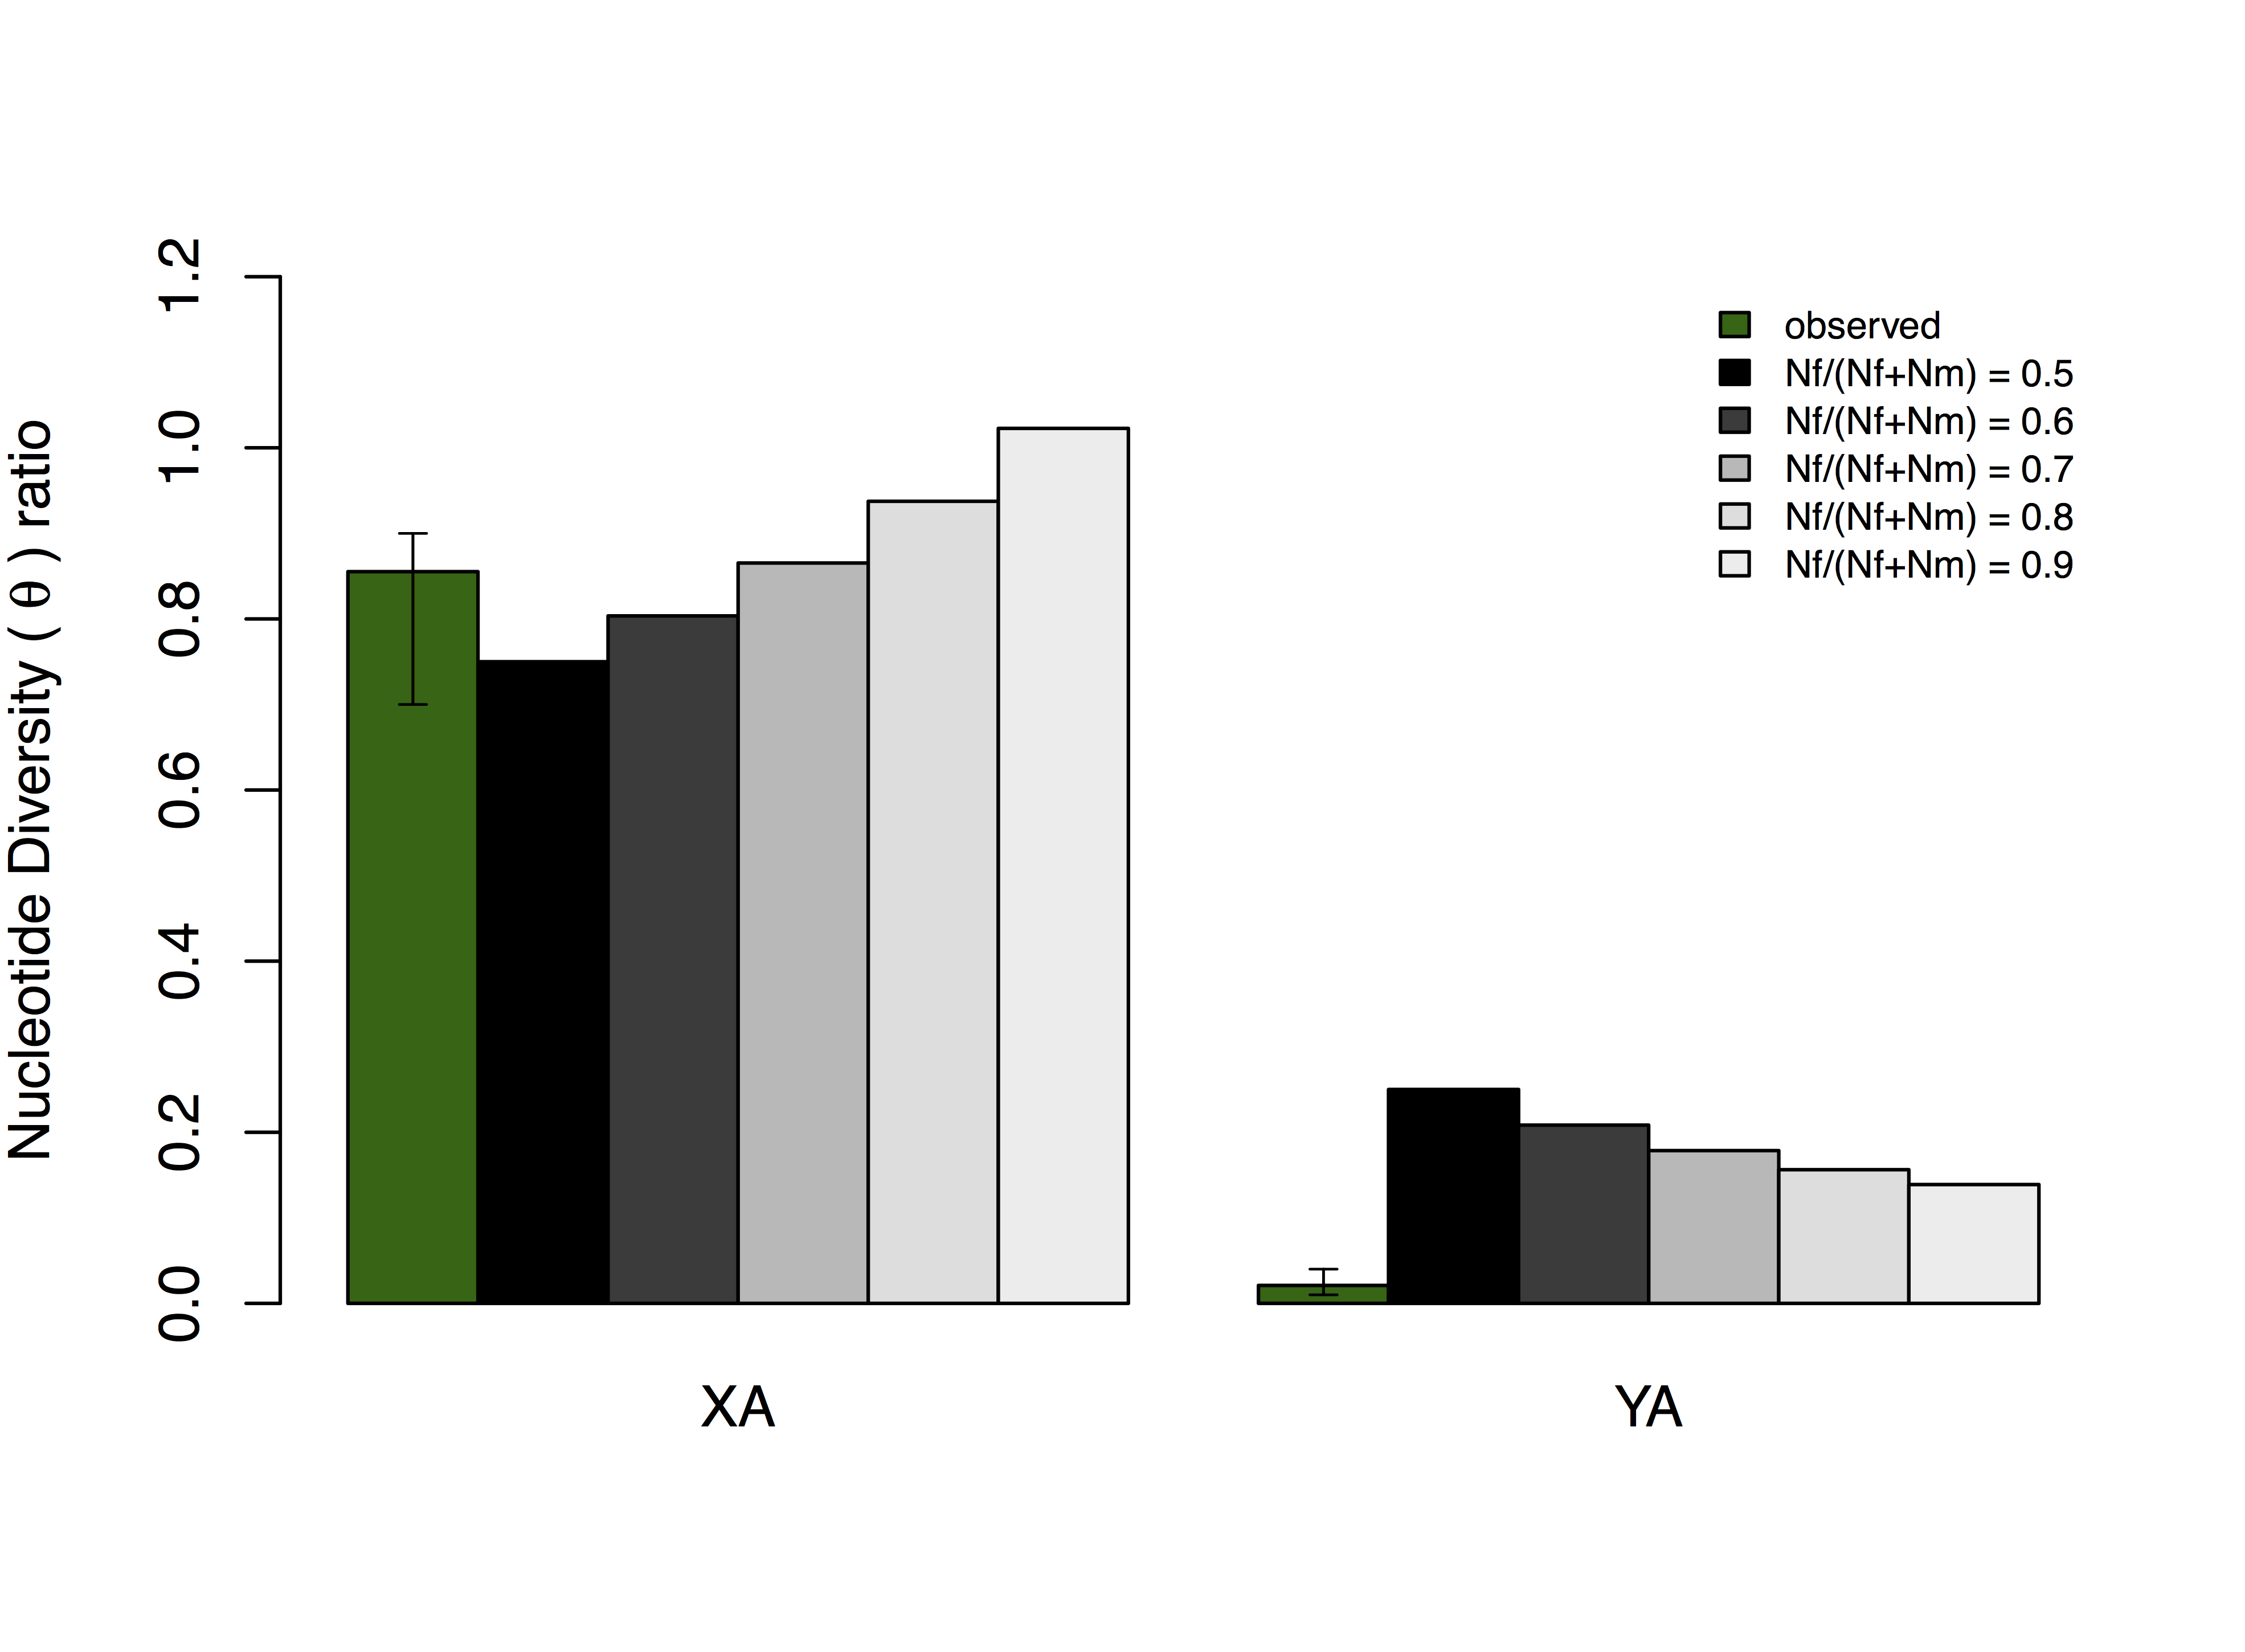
\includegraphics[width=\linewidth]{figure2.jpg}
%\caption{new figure coming soon).
%}
%\label{fig:spectrum}
%\end{figure}

\subsection*{Purifying selection}

\section*{Conclusions}

\section*{Acknowledgments}

\bibliography{bibliography}
\end{document}
